强化学习（RL）是推动大型基础模型走向自我改进的核心训练范式。本报告
介绍 MiMo-V2.6 系列，这是一个通过扩展 RL 算力推动模型智能前沿的全模态
家族。在 RL 之前，我们在广泛的多模态语料上进行中期训练，以提供充足的
探索空间，并在预训练的混合 SWA 架构上构建扎实的基础设施以支撑后续的
规模扩展。我们从三个维度扩展 RL 算力：（1）更大的批大小与更高的
吞吐，采用异步训练，每步消耗 1,568 个样本和 $2.7\sim$3.7B tokens，上下文
长度最高 1M；（2）更多样、更复杂的环境，在多种智能体脚手架的组合下
覆盖代码、通用、视觉和网络安全领域；（3）更多评分器算力，通过组内
智能体评分，为长程任务产出更准确的奖励信号，并引导模型走向更短、
更省 token 的解法。为在规模扩展下保持训练稳定，我们冻结 MoE 路由器，
并建立针对奖励作弊的多层防御。我们进一步构建混合任务智能体 RL 的
基础设施，包括统一的轨迹表示、高并发多框架 rollout、控制面与数据面
解耦，以及训练与推理的一致性。我们开源了训练动态、RL 环境和 RL 框架，
以促进复现以及关于规模化 RL 与模型自我改进的后续研究。







\begin{figure}[htbp]
\centering
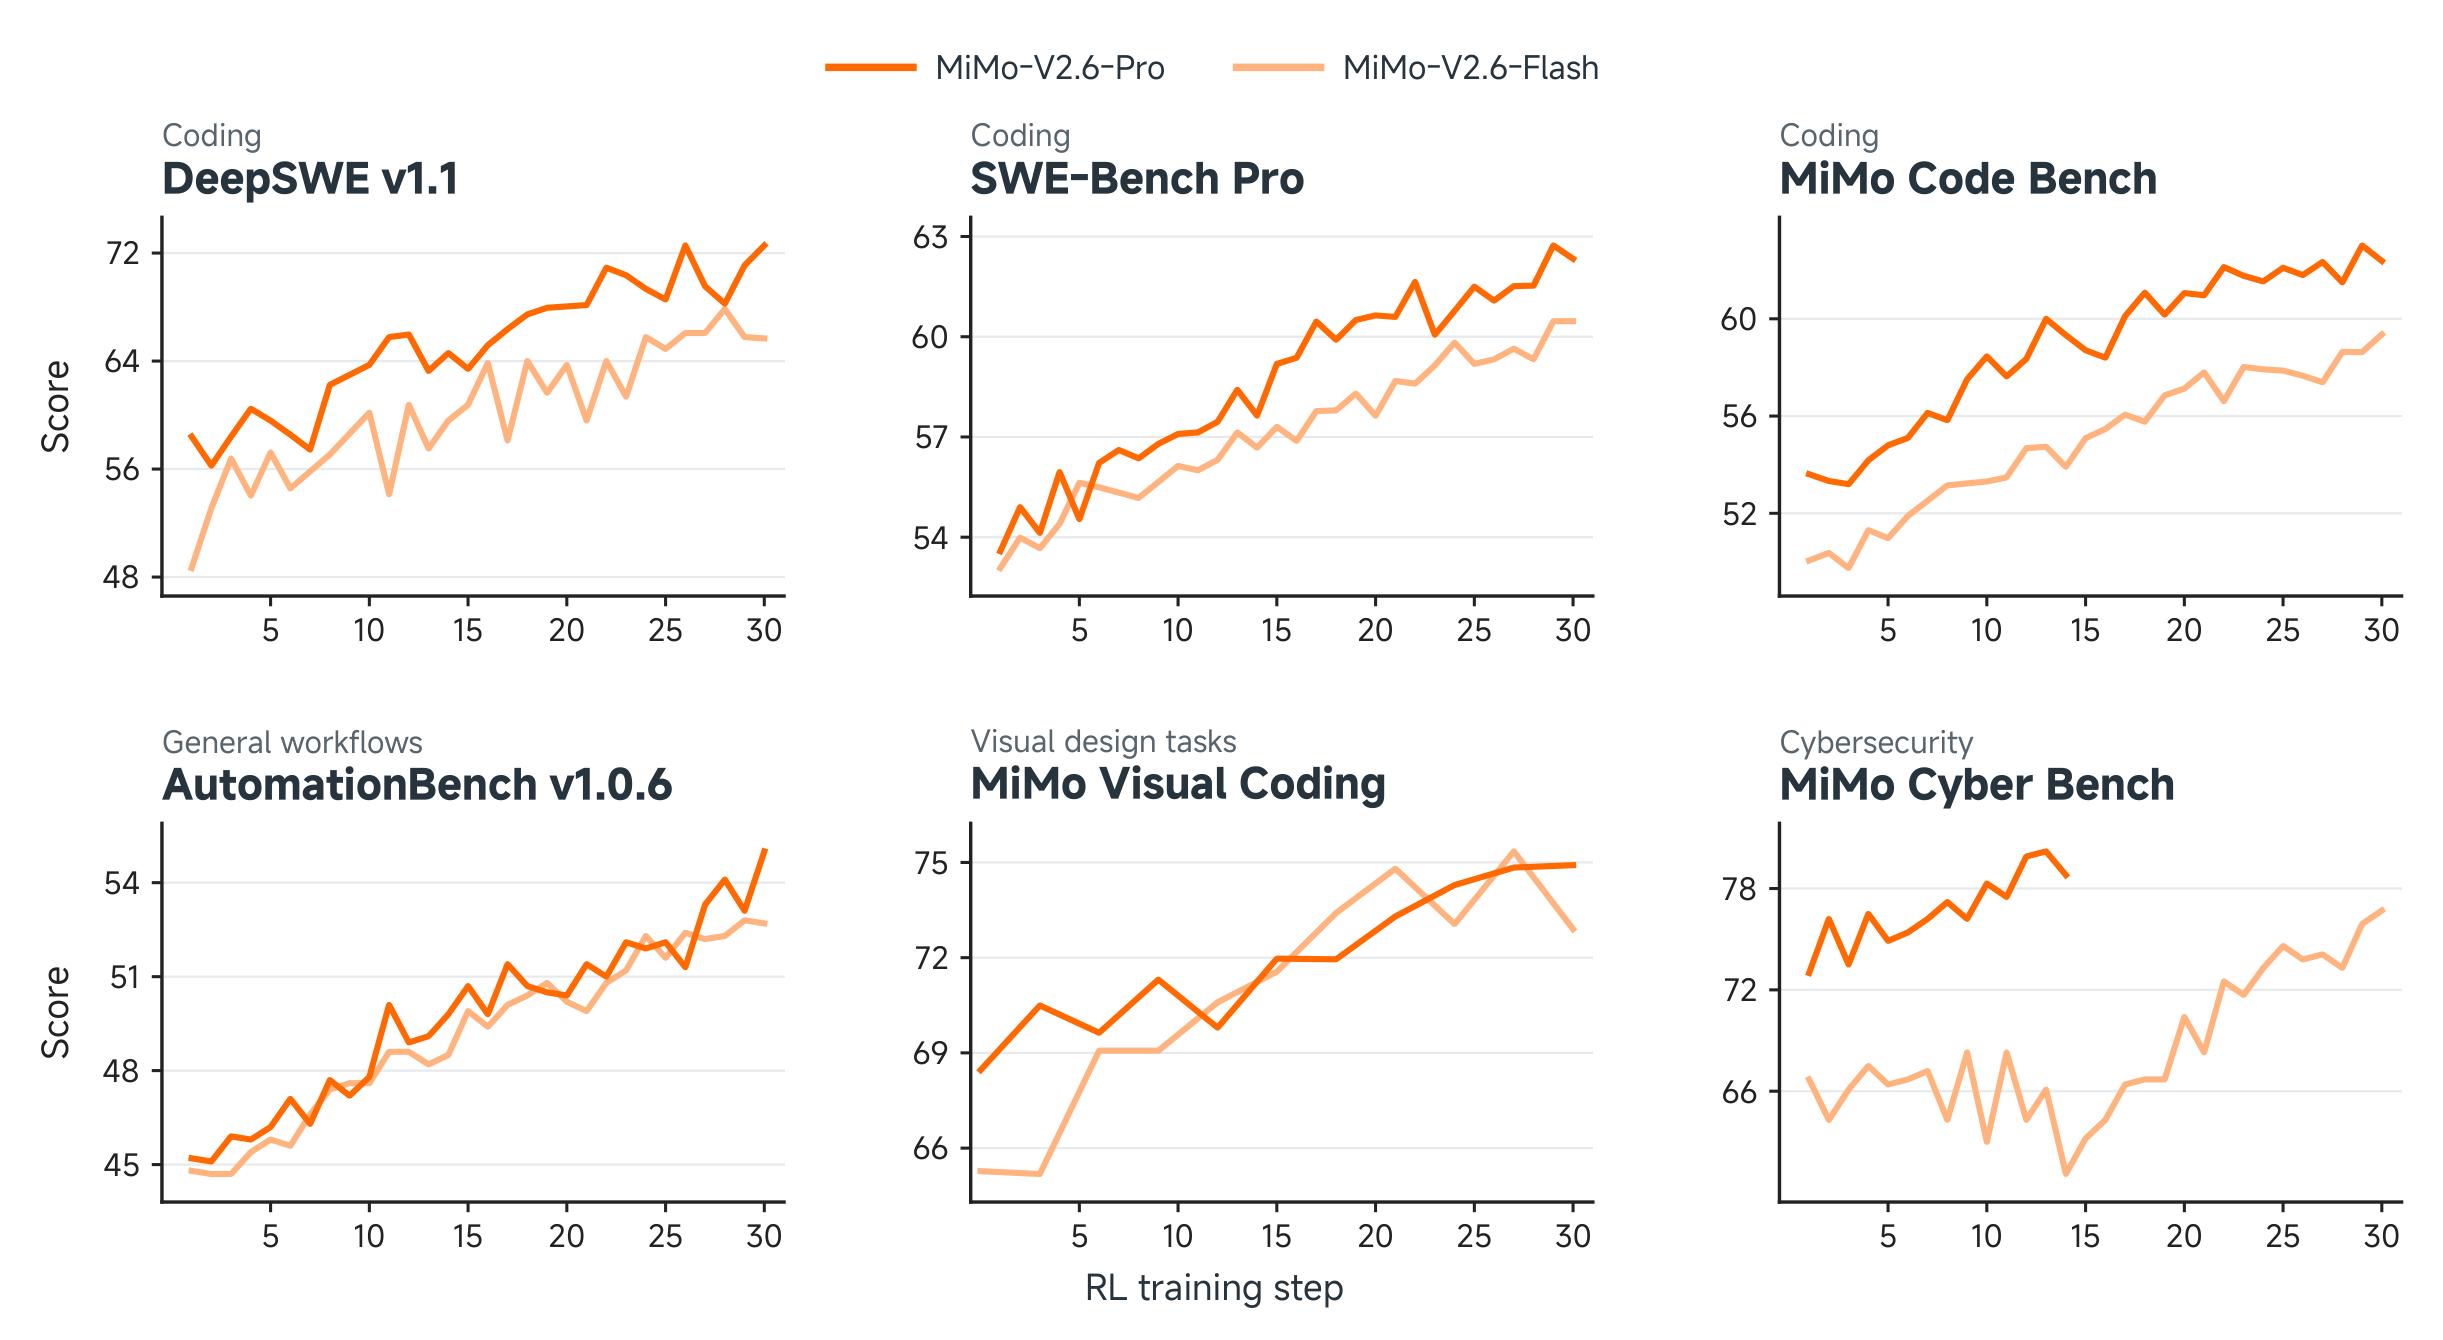
\includegraphics[width=\linewidth]{images_hi/fig01.png}
\caption{MiMo-V2.6-Pro 与 MiMo-V2.6-Flash 在整个 RL 训练过程中各任务的基准得分。}
\label{fig:1}
\end{figure}


\subsection{1 引言}\label{introduction}

递归自我改进（RSI）设想模型通过持续的探索与反馈来扩展自身能力。
实现这一愿景需要智能体，它们把模型与交互式环境耦合起来，从而提供
自我改进所依赖的多步轨迹和反馈信号。为此，在复杂的智能体任务上
扩展强化学习（RL）开辟了一条具体的路径。然而，释放这一潜力面临两大
挑战。第一，面向基础模型的 RL 需要合适的模型架构，以及为智能体提供
足够丰富的探索空间。第二，扩展 RL 需要基础设施、环境和评分器方面的
成熟方案。在本报告中，我们介绍 MiMo-V2.6 系列，包括 MiMo-V2.6-Pro——
一个 1.02T 参数、42B 激活参数的专家混合（MoE）模型，以及
MiMo-V2.6-Flash——一个 310B 参数、15B 激活参数的专家混合（MoE）模型，
以弥合这些差距，在规模化 RL 上迈出务实的一步。

MiMo-V2.6 的架构、预训练和中期训练共同构建了一个强大且高效的基础
模型。出于以低计算成本保留全局上下文的需要，MiMo-V2.6 构建了混合
稀疏 MoE Transformer 主干，将局部滑动窗口注意力（SWA）与全局注意力
（GA）交错排布，并辅以轻量视觉编码器和音频编码器。此外，大规模
预训练赋予模型广泛的知识，以及在文本、音频和视频上的多模态理解能力。
我们进一步引入以智能体为中心的中期训练阶段，扩展智能体任务的探索
空间，使模型在后训练期间能够发现更有效的解题轨迹。

接下来，我们通过一个系统化、协同设计的框架在三个关键组件上扩展 RL
算力。第一，我们通过全异步训练扩展批大小和训练吞吐，每步处理数千条
长程 rollout 和数十亿 token，上下文长度最高 1M。第二，我们扩展 RL
环境的多样性和复杂度，覆盖编码、通用、视觉和网络安全任务，使用
多样化的智能体脚手架，并加强对奖励作弊的防护。同时变化脚手架和任务
可以提升模型的泛化能力。第三，我们引入组内智能体评分，在二元测试
用例之外提供信息量更大的奖励信号。我们不再给所有通过测试用例的解法
分配相同奖励，而是在每个组内比较各解法，以区分解题质量和行为。通过
我们提出的组内奖励合成（GRS）和组内优势重分配（GAR），这些细粒度的
区分被转化为信息量更大的学习信号，引导模型走向更准确、更高效的解法。

在规模化实现这些，需要基础设施在研究和工程两方面应对挑战。为支持
灵活的智能体交互场景，我们设计了统一的轨迹表示和惩罚机制，二者共同
精炼学习信号。为处理大训练批，我们通过脚手架池在多种智能体框架间
维持高并发交互，并将控制面与数据面解耦，以缓冲和传输携带路由与
多模态负载的海量轨迹。样本混合机制与动态采样和部分 rollout 协同工作，
稳定训练批中每个任务的样本组成。我们在 MoE 路由和 top-p 采样的候选
集合上对齐训练与推理引擎，并针对 RL 负载优化两个引擎。

扩展 RL 算力显著释放了模型在可验证任务（如编码）和较难验证任务
（如网页开发）上的潜力。如图 1 所示，随着训练步数增加，MiMo-V2.6-Pro
和 MiMo-V2.6-Flash 在所报告的基准上均稳步提升。而且这些收益并不局限
于单一领域，而是在多样任务上一致成立，涵盖 DeepSWE
（Huang et al., 2026）上的编码、AutomationBench
（Shepard and Salimans, 2026）上的通用工作流、MiMo Visual Coding 上的
视觉任务，以及 MiMo Cyber Bench 上的网络安全。这些收益表明，
MiMo-V2.6 具备更强的复杂问题求解能力，在日常协同工作场景中表现更
可靠，体现出更通用的智能体智能。

为促进智能体 RL 的研究，我们开源了一套覆盖 RL 开发栈关键组件的综合
套件，包括轻量模型 MiMo-V2.6-Distill-Qwen-9B、带校验器的多领域精选
任务环境、端到端 RL 训练框架，以及用于灵活智能体交互的可组合
mini-harness。这些组件共同为在多样任务、环境和智能体配置下研究智能体
RL 提供了统一且易用的平台，同时降低了复现和扩展大规模 RL 实验的工程
门槛。在 MiMo-V2.6-Distill-Qwen-9B 上的实验表明，RL 在多样任务和智能体
脚手架上均带来一致的收益，验证了所提套件的有效性和通用性。我们希望
这套开源套件能成为社区公平、强大且可复现的基线，支持对智能体 RL 的
系统性研究，并推动面向递归自我改进的研究。

\subsection{2 架构}\label{architecture}

\subsection{2.1 整体架构}\label{overall-architecture}

如图 2 所示，MiMo-V2.6 采用标准 Transformer（Vaswani et al., 2017）
主干，并辅以通过轻量投影器连接的视觉编码器和音频编码器。

MiMo-V2.6 的文本主干主要由重复的混合块组成，这些块将局部滑动窗口
注意力（SWA）与全局注意力（GA）交错排布。它堆叠 $M$ 个混合块，每个
块由 $N$ 个连续的 SWA 块后接一个 GA 块构成。唯一的例外是最开始的
Transformer 块，它使用带稠密前馈网络（FFN）的全局注意力，以稳定早期的
表示学习。MiMo-V2.6 中使用的滑动窗口大小 $W$ 为 128。SWA 块和 GA 块
都使用不带共享专家的稀疏 MoE FFN。MiMo-V2.6 还集成了基于 SWA 和稠密
FFN 的 MTP（Gloeckle et al., 2024; Liu et al., 2024; Xia et al., 2025），
以在预训练期间提升模型性能。关于文本主干架构更全面的描述可参见
Core Team et al.~(2026)。模型配置见表 1。
